\begin{flushright}
                      از درس مبانی‌ مدارهای الکتریک، ترانزیستورها را بیاد می‌آوریم.
                      مدار زیر متشکل از دو ترانزیستور MOSFET می‌باشد.

                      \begin{figure}[h]
                          \centering
                          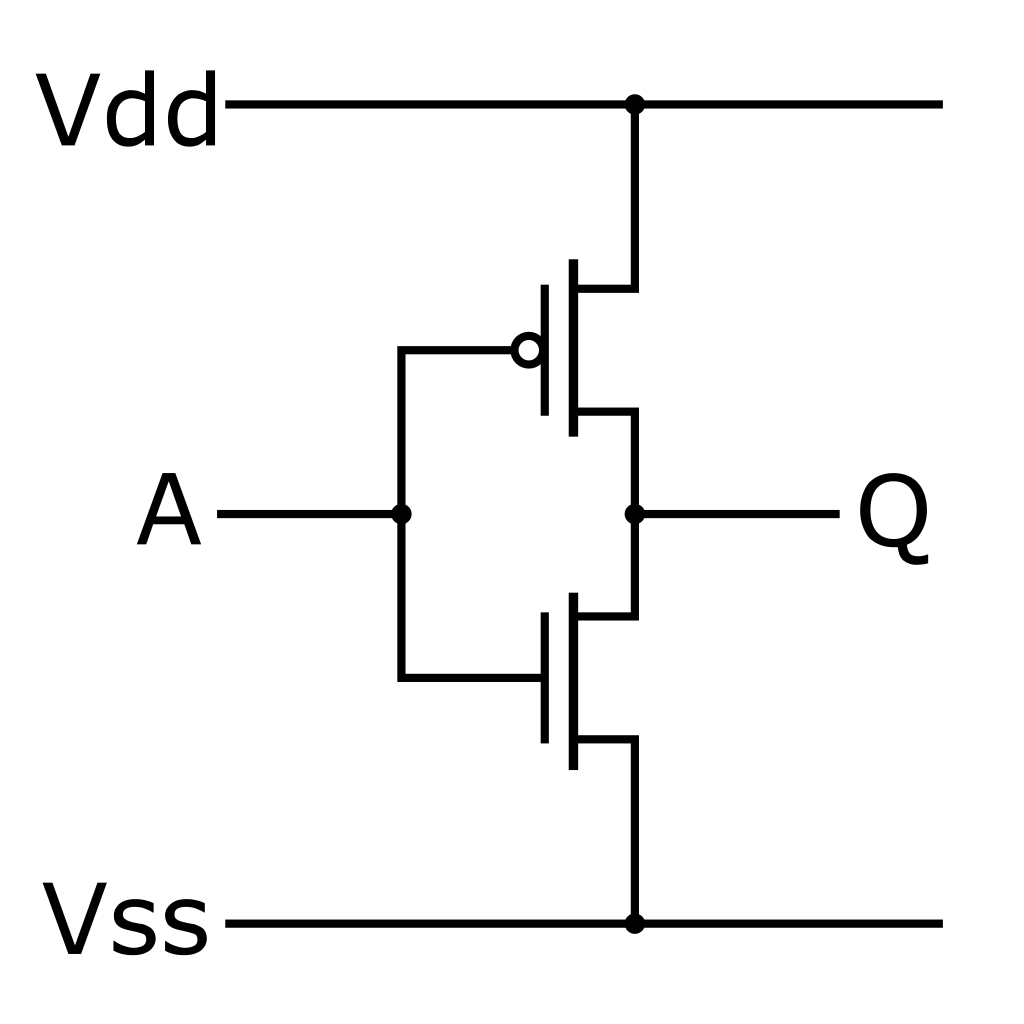
\includegraphics[width= 0.4\textwidth]{source/not-gate-imp}
                          \caption{پیاده‌سازی گیت not}
                          \label{fig:not-gate-imp}

                      \end{figure}

                      همانطور که به یاد دارید، این مدار در صورتی که ولتاژ ورودی بالا داشته باشد،
                      $v_{ss}$
                      را خروجی می‌دهد و در صورتی که ولتاژ ورودی پایینی داشته باشد،
                      $v_{dd}$
                      را خورجی می‌دهد.

                      در نگاه \textbf{انتزاعی} با در نظر گرفتن یک محدوده ولتاژ برای 1 و 0 منطقی، می‌توان آن را به چشم یک گیت not منطقی در نظر گرفت.
                      یا به بیان دیگر، شکل 1 یک \textbf{پیاده‌سازی} از گیت not منطقی می‌باشد.

                      \begin{figure}[h]
                          \centering
                          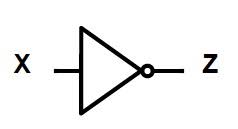
\includegraphics[width= 0.4\textwidth]{source/not-gate-abs}
                          \caption{انتزاعی از مدار متشکل از دو ترانزیستور}
                          \label{fig:not-gate-abs}
                      \end{figure}

\end{flushright}

